\newpage
\section*{CHAPTER 4. EXPERIMENTAL RESULTS}
\phantomsection\addcontentsline{toc}{section}{CHAPTER 4. EXPERIMENTAL RESULTS}
\setcounter{section}{4}
\setcounter{subsection}{0}
\setcounter{subsubsection}{0}
\setcounter{paragraph}{0}
\setcounter{figure}{0}
\setcounter{table}{0}

Chapter 4 presents the experimental procedure and evaluation results of the proposed quantized HiFiC GAN accelerator. Following an evaluation-oriented structure, this chapter first describes the accuracy evaluation environment and the quantization results, then reports FPGA resource utilization, analyzes performance, compares the hardware-oriented implementation with the software reference, and finally summarizes the main observations.

%%%%%%%%%%%%%%%%%%%%%%%%%%%%%%%%%%%%%%%%%%%%%%%%%%%%%%%%%%%%%%%%%%%%%%%%%%%%%%%%%%%
\subsection{Accuracy Evaluation}

The first objective of the evaluation is to verify that the hardware-oriented implementation preserves the functional behavior of the HiFiC inference pipeline. Since the proposed accelerator implements the complete generator, the verification process compares the HLS/FPGA-oriented output with the Python reference model using the same input tensors and model parameters.

\subsubsection{Verification Environment}

The overall testing methodology is shown in Figure~\ref{fig:testing_env}. A set of test images ($256 \times 256$ RGB) drives two paths in parallel: the proposed HiFiC GAN accelerator running on the ZCU104 FPGA (the design under test) and a reference model, namely the original HiFiC FP32 network implemented in Python/PyTorch. For each test item, the accelerator output is compared against the reference output to produce a PASS/FAIL verdict for hardware behavior verification, while the reconstructed images are compared to quantify quality and performance through metrics such as speedup, PSNR/SSIM, latency, and compression ratio.

\begin{figure}[H]
    \centering
    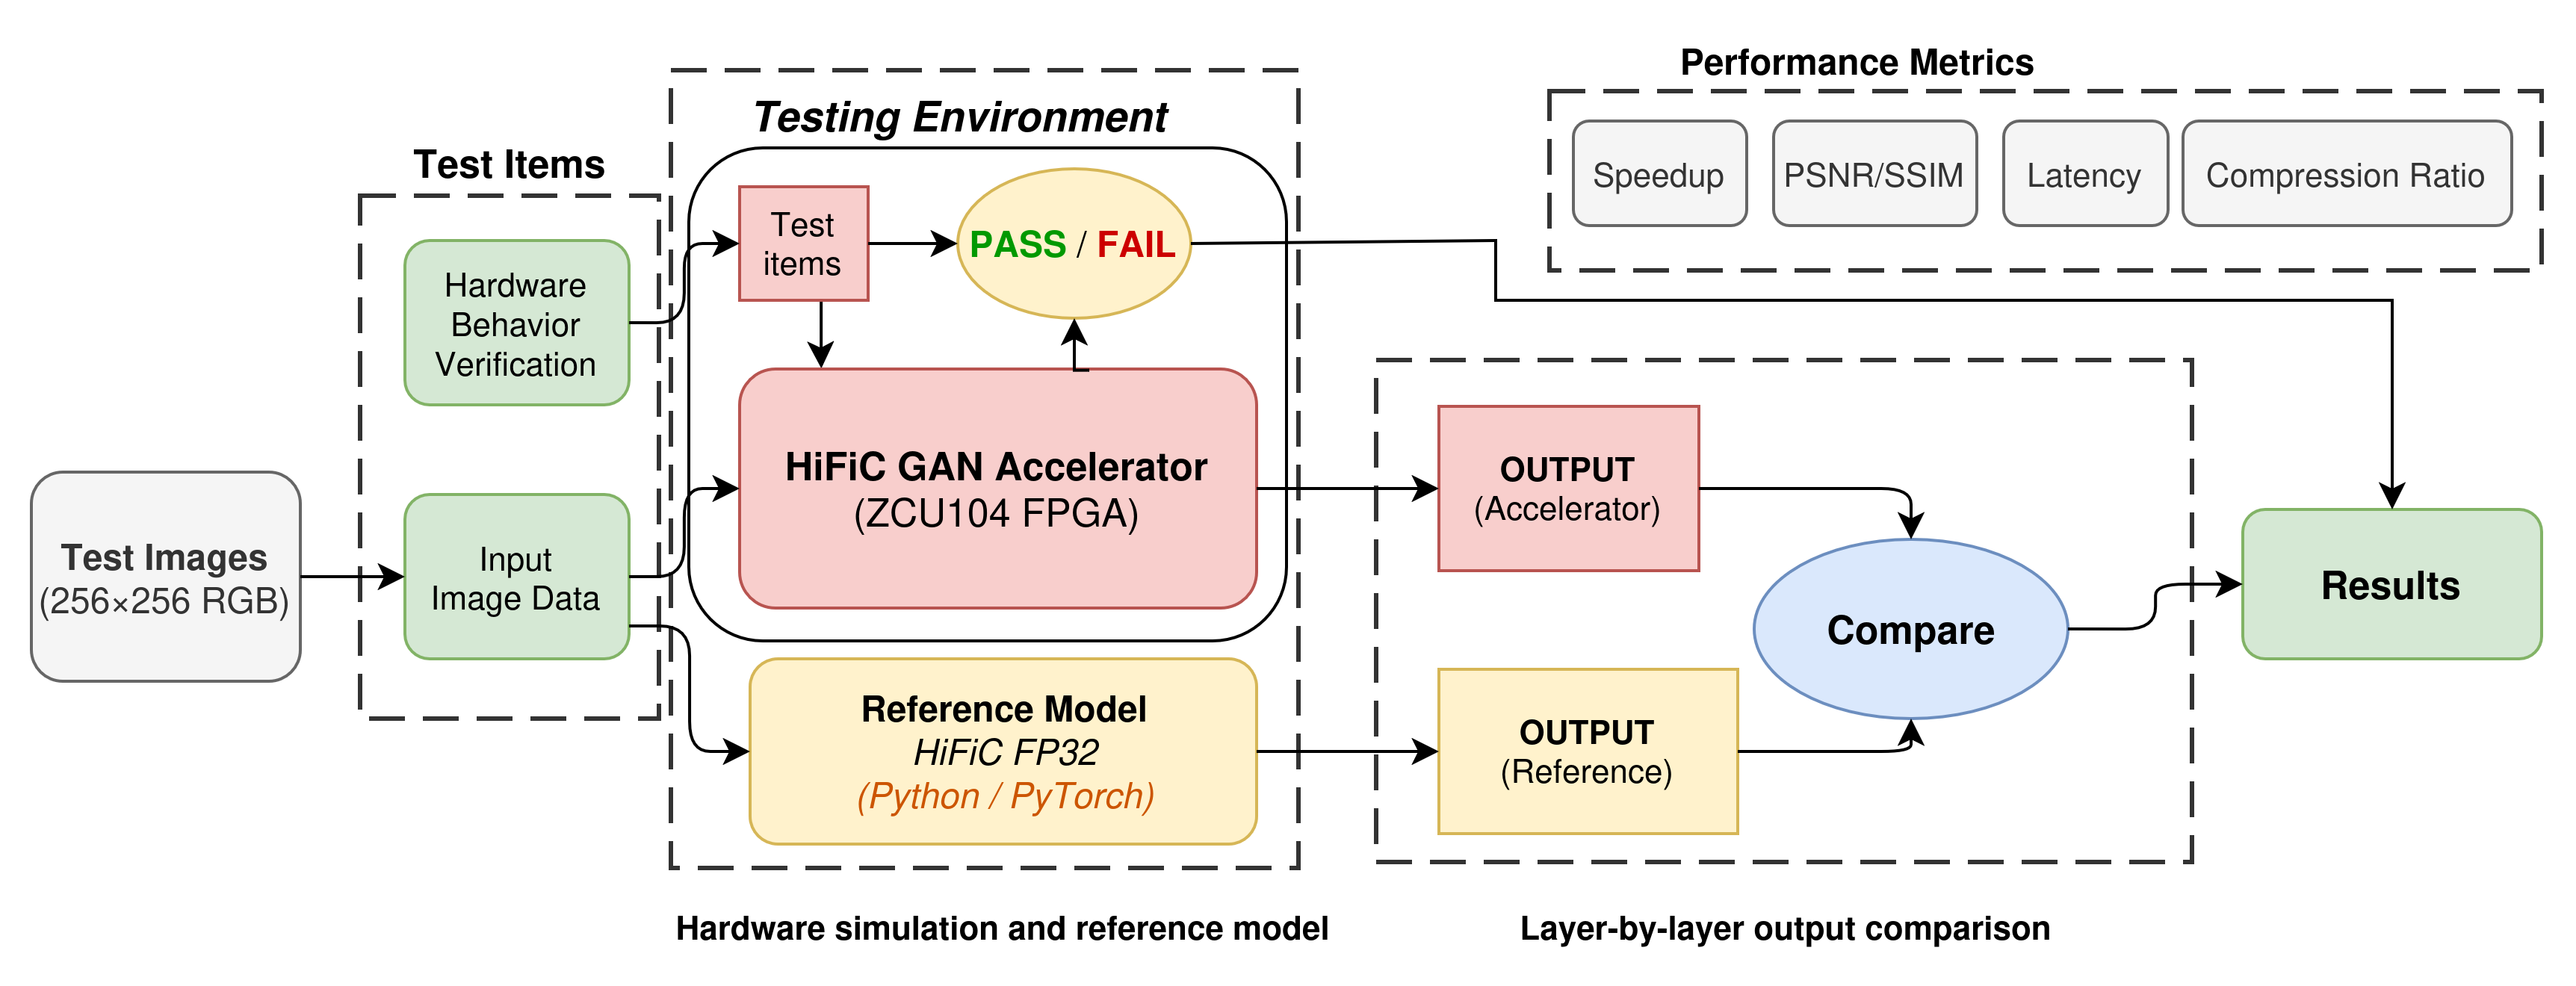
\includegraphics[width=\textwidth]{Images/testing_env.png}
    \caption{Testing environment: the accelerator under test compared against the HiFiC FP32 reference model}
    \label{fig:testing_env}
\end{figure}

Figure~\ref{fig:system_architecture} illustrates the verification and deployment environment used in this thesis. The system follows a hardware--software co-design approach on the ZCU104 platform. The Processing System (PS) is responsible for software control, memory management, and accelerator invocation, while the Programmable Logic (PL) implements the custom generator accelerator.

\begin{figure}[H]
    \centering
    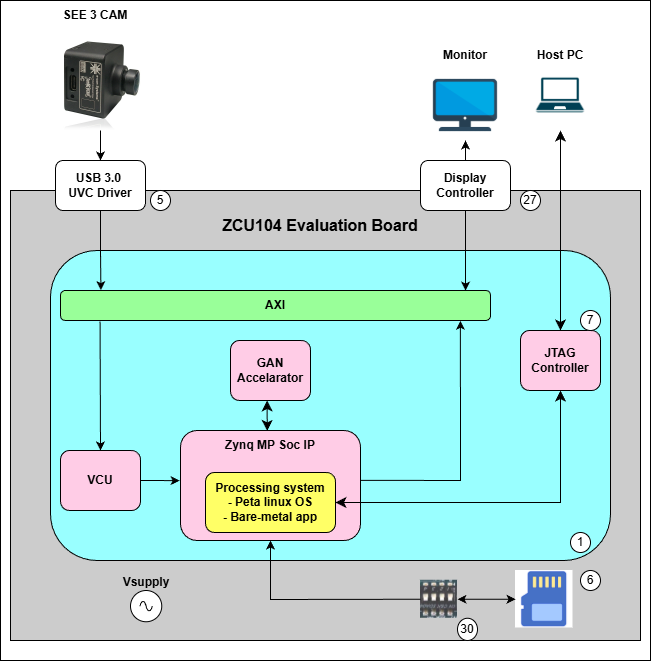
\includegraphics[width=1\linewidth]{Images/System Architecture.png}
    \caption{Verification and deployment environment on the ZCU104 platform}
    \label{fig:system_architecture}
\end{figure}

The software reference is executed in Python to generate golden outputs for comparison. The same input tensors, weights, and normalization parameters are then used by the HLS C/C++ implementation. During simulation, the output of the HLS model is compared with the Python reference to verify numerical consistency. After successful HLS verification, the generated IP core is integrated into the Vivado block design shown in Figure~\ref{fig:vivado_block_design}.

\begin{figure}[H]
    \centering
    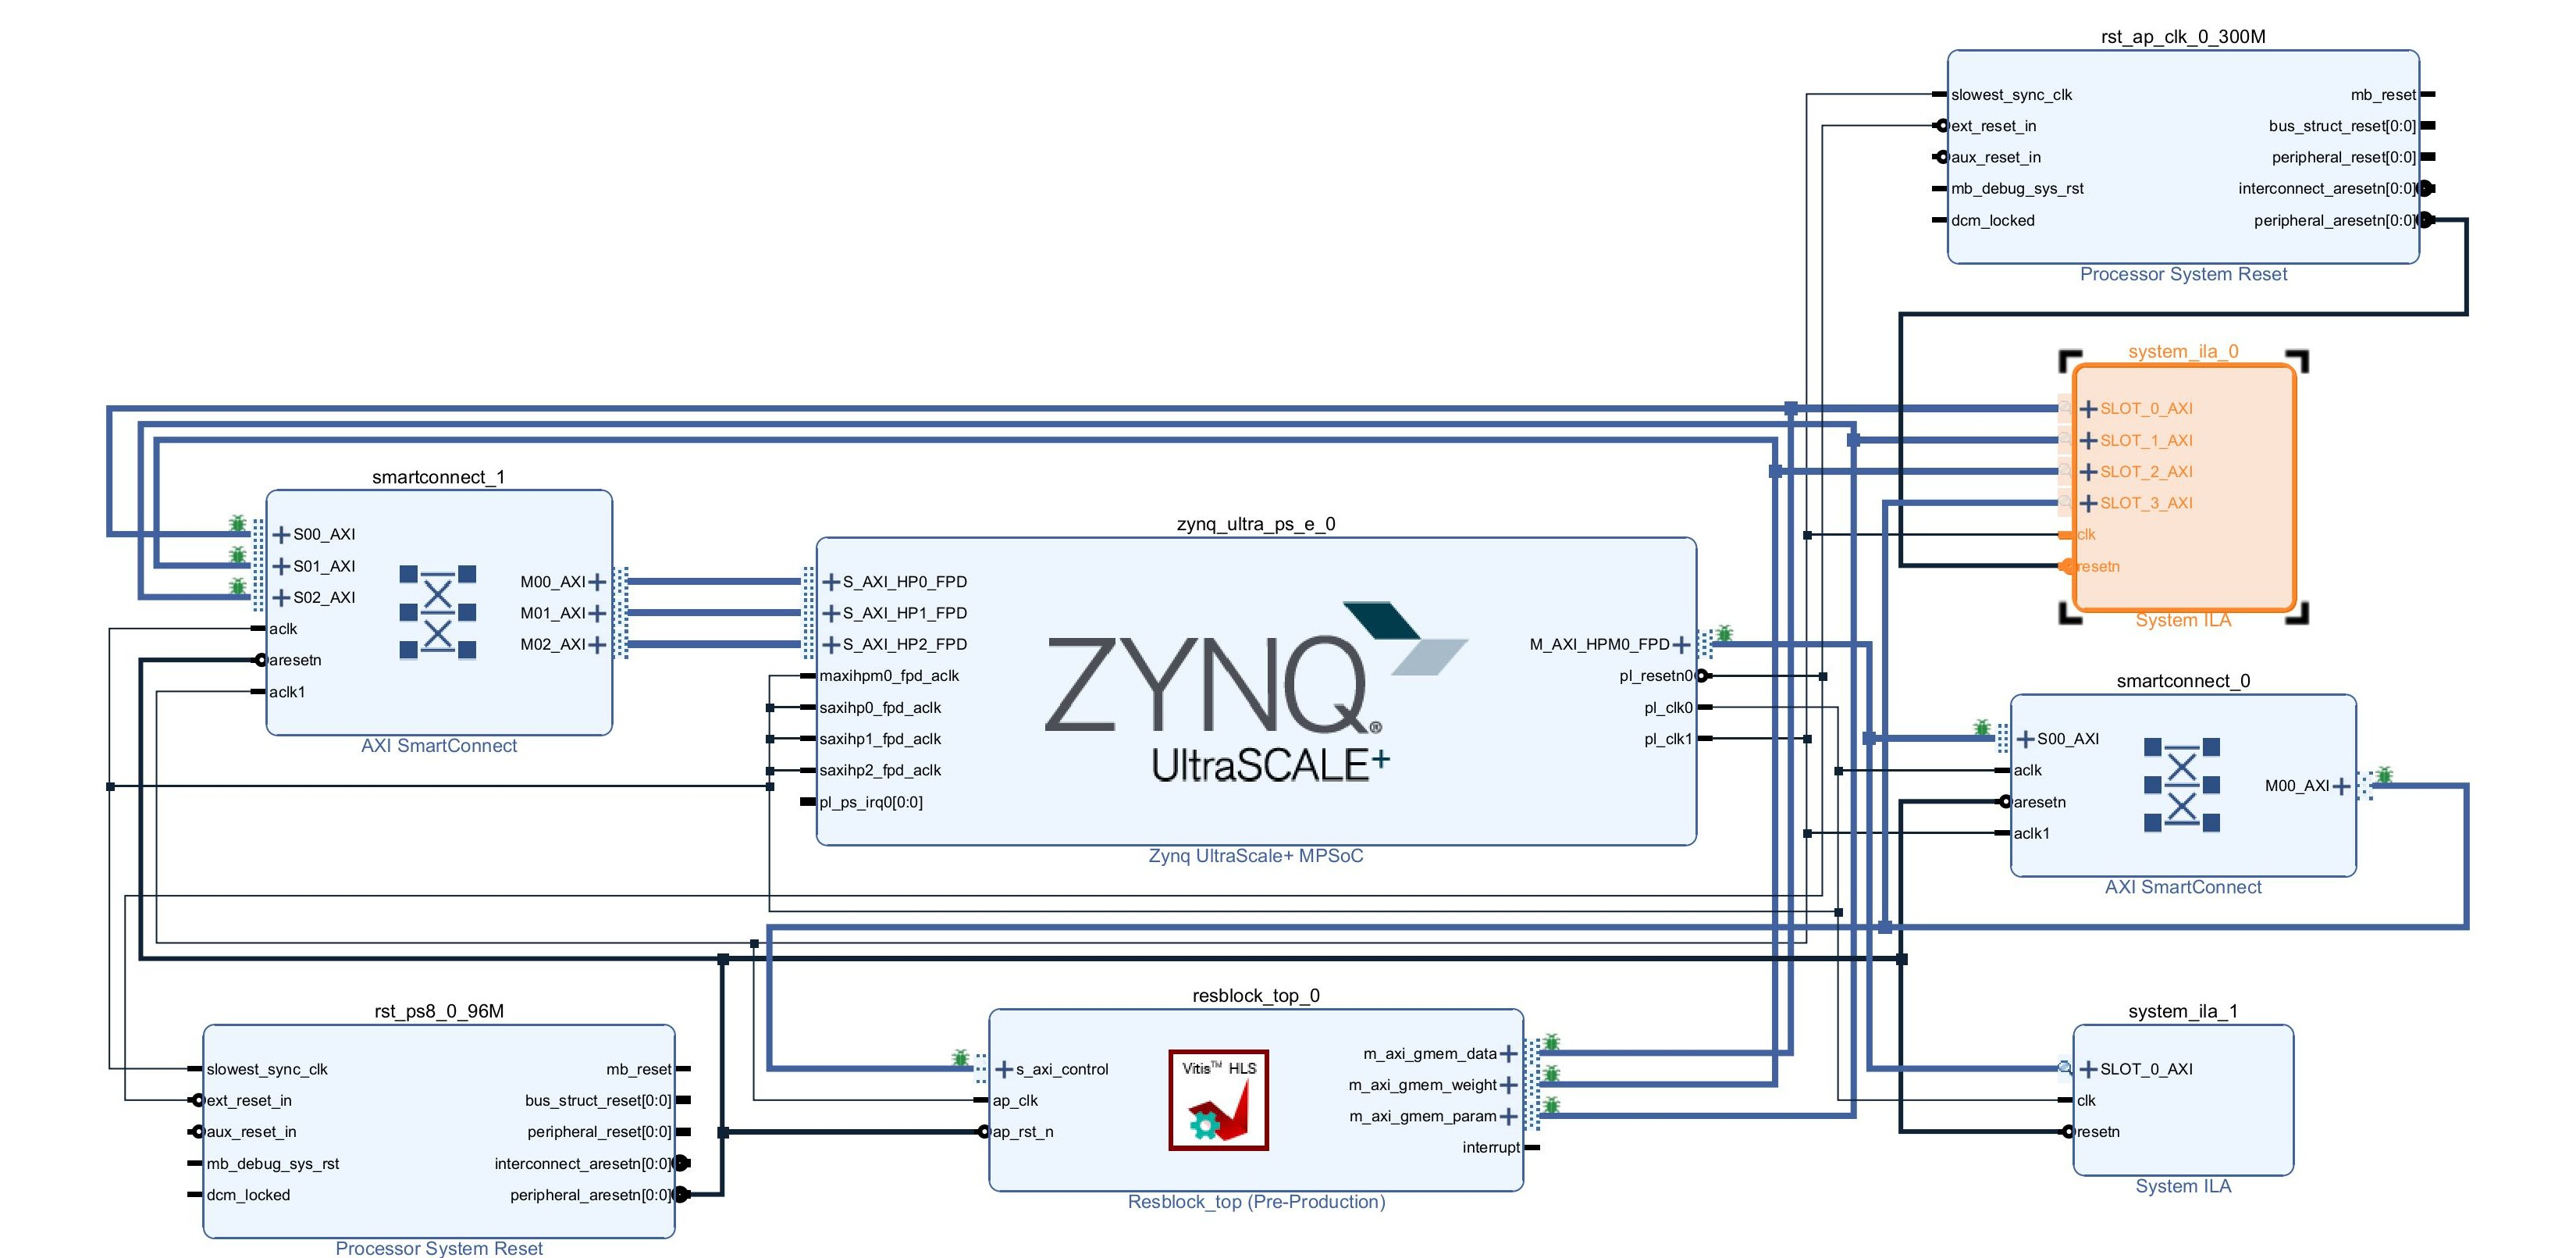
\includegraphics[width=1\linewidth]{Images/block_design.jpg}
    \caption{Vivado block design of the proposed accelerator system}
    \label{fig:vivado_block_design}
\end{figure}

The target board used for implementation is the Zynq\texttrademark{} UltraScale+\texttrademark{} MPSoC ZCU104, shown in Figure~\ref{fig:ZCU}. The most relevant components for this thesis are summarized in Table~\ref{tab:zcu104_components}. These components provide the processing system, programmable logic, external memory, SD-card boot interface, and display/output connections required for testing the accelerator.

\begin{figure}[H]
    \centering
    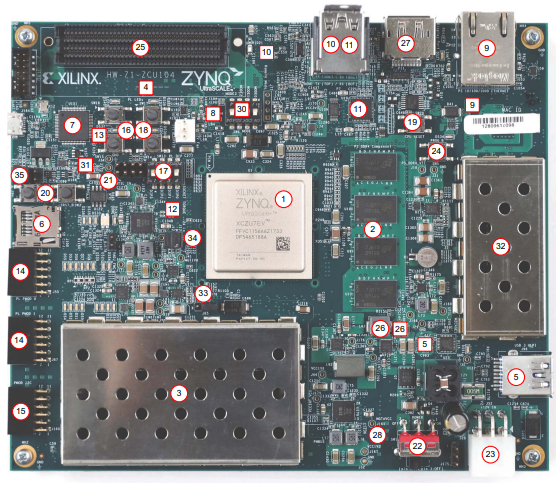
\includegraphics[width=0.9\linewidth]{Images/ZCU.png}
    \caption[Zynq\texttrademark{} UltraScale+\texttrademark{} MPSoC ZCU104 evaluation board]{Zynq\texttrademark{} UltraScale+\texttrademark{} MPSoC ZCU104 evaluation board \cite{xilinx2018zcu104}}
    \label{fig:ZCU}
\end{figure}

\begin{table}[H]
    \centering
    \caption[Relevant ZCU104 components for accelerator evaluation]{Relevant ZCU104 components for accelerator evaluation (the item numbers follow the board component callouts in the ZCU104 user guide~\cite{xilinx2018zcu104})}
    \label{tab:zcu104_components}
    \begin{tabular}{|c|l|}
        \hline
        \textbf{No.} & \textbf{Component} \\
        \hline
        1 & Zynq UltraScale+ XCZU7EV MPSoC \\
        \hline
        3 & PL-side SODIMM DDR4 memory \\
        \hline
        5 & USB 3.0 transceiver and USB 2.0 ULPI PHY \\
        \hline
        6 & SD-card interface connector \\
        \hline
        7 & Programmable Logic JTAG \\
        \hline
        27 & DisplayPort connector \\
        \hline
    \end{tabular}
\end{table}

The verification flow consists of four main steps. First, the Python reference model produces the expected reconstructed output or intermediate feature output. Second, the HLS C/C++ model processes the same input data using the hardware-oriented implementation. Third, the two outputs are compared using objective image-quality metrics. Finally, after synthesis and implementation, the accelerator is controlled from Vitis on the ZCU104 platform to measure board-level behavior.

\subsubsection{Functional Verification Results}

Before board-level deployment, the hardware-oriented C/C++ model of every generator stage was validated against the FP32 golden tensors exported from the original HiFiC model through C-simulation (CSIM). A block is considered to PASS when its maximum absolute error stays below the tolerance assigned to that stage and no output element is reported as a mismatch. Table~\ref{tab:csim_verification} summarizes the block-level results obtained on real input data.

\begin{table}[H]
\centering
\caption{Block-level functional verification (CSIM) against the FP32 golden reference}
\label{tab:csim_verification}
\small
\renewcommand{\arraystretch}{1.2}
\begin{tabular}{|l|c|c|c|c|}
\hline
\textbf{Block} & \textbf{Tensor shape (in $\rightarrow$ out)} & \textbf{Max abs. error} & \textbf{RMSE} & \textbf{Mismatch} \\
\hline
CBI & $16\times16\times220 \rightarrow 960$ & 0.01953 & 0.00169 & 0 / 245,760 \\
\hline
ResBlock & $16\times16\times960 \rightarrow 960$ & 0.01953 & 0.000978 & 0 / 245,760 \\
\hline
GlobalAdd & $16\times16\times960$ & 0.02344 & 0.00178 & 0 / 245,760 \\
\hline
UCB\_0 & $16\times16\times960 \rightarrow 32\times32\times480$ & 0.00781 & 0.000591 & 0 / 491,520 \\
\hline
UCB\_1 & $32\times32\times480 \rightarrow 64\times64\times240$ & 0.01367 & 0.001061 & 0 / 983,040 \\
\hline
UCB\_2 & $64\times64\times240 \rightarrow 128\times128\times120$ & 0.02148 & 0.002284 & 0 / 1,966,080 \\
\hline
UCB\_3 & $128\times128\times120 \rightarrow 256\times256\times60$ & 0.01563 & 0.001405 & 0 / 3,932,160 \\
\hline
Conv77 & $256\times256\times60 \rightarrow 3$ & 0.488 & 0.162 & 0 / 196,608 \\
\hline
\end{tabular}
\end{table}

Every block passes with zero element mismatches, which confirms that the mixed-precision FP16 datapath reproduces the reference behavior of the generator. For all feature-map stages the error magnitude is small, with an RMSE on the order of $10^{-3}$. The Conv77 output is evaluated with a relaxed tolerance because its final \texttt{Clip}$(0,1)$ together with the FP16 accumulation over a $7\times7$ window produces a slightly larger but still visually negligible deviation, which is further confirmed by the image-quality metrics reported in the following subsections.

\subsubsection{Test Images and Evaluation Metrics}

The evaluation uses representative RGB images resized to $256 \times 256$, consistent with the input size used throughout this thesis. The reconstructed images are evaluated using image-quality metrics introduced in Chapter~2, including Peak Signal-to-Noise Ratio (PSNR), Structural Similarity Index Measure (SSIM), Learned Perceptual Image Patch Similarity (LPIPS), and Mean Squared Error (MSE). These metrics are suitable for checking whether the quantized hardware-oriented implementation remains close to the software reference.

Figure~\ref{fig:chapter4_psnr_comparison} shows the PSNR comparison between the Python reference model and the HLS simulation model over 100 test images. The similarity of the two curves indicates that the HLS implementation follows the numerical behavior of the reference model closely enough for FPGA deployment.

\begin{figure}[H]
    \centering
    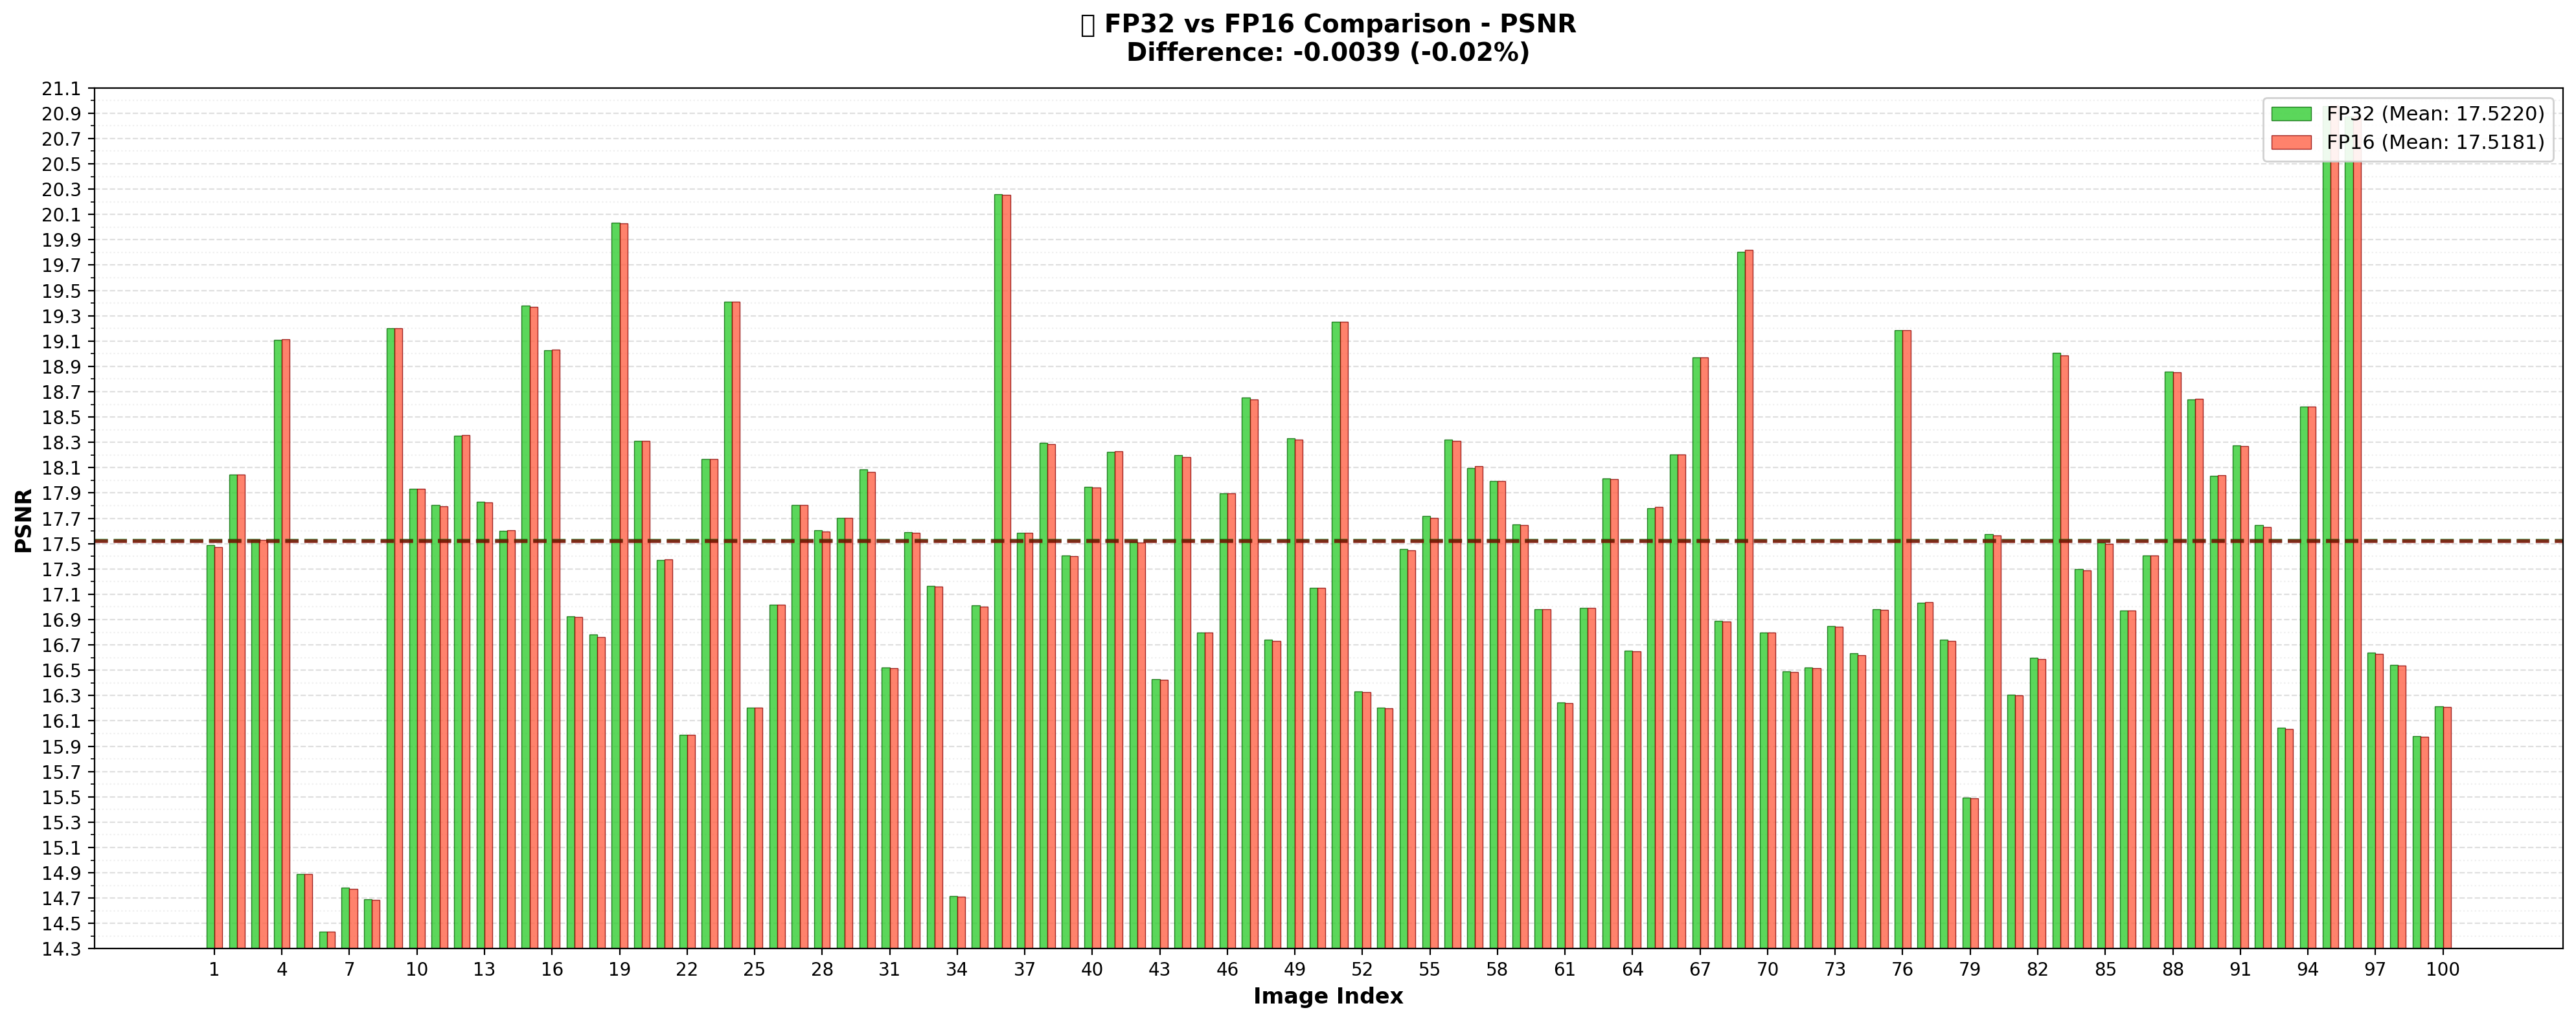
\includegraphics[width=1\linewidth]{Images/comparison_psnr_sidebyside.png}
    \caption{PSNR comparison between the Python reference model and the quantized HLS simulation model}
    \label{fig:chapter4_psnr_comparison}
\end{figure}

Overall, the accuracy evaluation confirms that the hardware-oriented ResBlock implementation preserves the main reconstruction behavior of the HiFiC generator. Small numerical differences are expected because the accelerator uses a mixed-precision data path, but the observed quality trend remains close to the Python reference.

\subsubsection{Mixed-Precision Quantization Results}

This subsection evaluates the impact of the mixed-precision quantization described in Chapter~3, i.e., the transition from full-precision FP32 computation to a mixed-precision FP16 implementation, on compression efficiency and reconstructed image quality. The experiment uses a representative test image with a resolution of $256 \times 256$. Two configurations are compared under identical conditions: the baseline FP32 model and the quantized mixed-precision FP16 model, where internal computations operate in FP16 while input and output interfaces remain in FP32. Table~\ref{tab:quant_results} summarizes the quantitative compression metrics obtained from both models.

\begin{table}[H]
\centering
\caption{Comparison between FP32 and FP16 mixed-precision HiFiC models}
\label{tab:quant_results}
\begin{tabular}{|l|c|c|c|}
\hline
\textbf{Metric} & \textbf{FP32} & \textbf{FP16 Mixed} & \textbf{Delta} \\
\hline
Original Size (bytes) & 25,879 & 25,879 & 0 \\
Bitstream Size (bytes) & 6,522 & 6,517 & -5 \\
Output Image Size (bytes) & 97,596 & 97,496 & -100 \\
Compression Ratio & 3.97$\times$ & 3.97$\times$ & 0.00 \\
Space Saving (\%) & 74.80 & 74.82 & +0.02 \\
Bits Per Pixel (bpp) & 0.7961 & 0.7955 & -0.0006 \\
PSNR (dB) & 19.08 & 19.05 & -0.03 \\
SSIM & 0.8315 & 0.8314 & -0.0001 \\
LPIPS & 0.0913 & 0.0925 & +0.0012 \\
MSE  &  804.315755 & 808.560496 & 4.244 \\
\hline
\end{tabular}
\end{table}

The results indicate that the compression performance of the HiFiC model is preserved after quantization. The bitstream size is slightly reduced, while the compression ratio and space-saving metrics remain unchanged. This suggests that the probability distribution of the latent representation is not significantly affected by FP16 rounding errors, allowing the entropy coding process to operate efficiently. From a perceptual quality perspective, the degradation introduced by mixed-precision computation is negligible: the observed PSNR reduction of 0.03~dB is well below the threshold of perceptual visibility, the SSIM metric remains nearly identical, and the LPIPS perceptual distance rises by only 0.0012 (from 0.0913 to 0.0925) between the two configurations.

The absolute PSNR reported here (19.08~dB) is noticeably lower than the $\sim$28.5~dB listed for HiFiC in the survey of Table~\ref{tab:model_survey}. This gap is not caused by quantization---the FP32$\rightarrow$FP16 difference is only 0.03~dB---but by the different evaluation conditions. The survey value is a dataset-averaged figure reported in the original HiFiC paper on standard benchmarks at $\sim$0.4~bpp, whereas the value here is measured on 100 test images of $256\times256$. Because HiFiC is optimized for perceptual quality rather than pixel-wise distortion, its PSNR is inherently modest and strongly content-dependent, so a single textured image can score well below the dataset average while remaining perceptually faithful, as confirmed by the visual comparison in Figure~\ref{fig:quant_visual}, the high SSIM of 0.83, and especially the low LPIPS of 0.0913---in line with, and even slightly better than, the $\sim$0.15 dataset-averaged LPIPS reported for HiFiC in Table~\ref{tab:model_survey}---which together evidence strong perceptual fidelity despite the modest PSNR. To strengthen the statistical reliability of the absolute quality figures, this measurement should be repeated over a larger image set (at least three images) in future work; the single-image measurement is sufficient for its purpose here, which is to isolate the FP32-versus-FP16 quantization delta.

Figure~\ref{fig:quant_visual} provides a visual comparison between the reconstructed images produced by the FP32 and FP16 models. No visible artifacts or structural distortions are observed in the quantized output, confirming that the proposed mixed-precision quantization strategy achieves a favorable balance between numerical efficiency and output fidelity.

\begin{figure}[H]
    \centering
    
\includegraphics[width=0.45\linewidth]{Images/originial.png}
    \hfill
    
\includegraphics[width=0.45\linewidth]{Images/quantized picture.png}
    \caption{Visual comparison of reconstructed images: FP32 model (left) and FP16 mixed-precision model (right)}
    \label{fig:quant_visual}
\end{figure}

% =====================================================================
% NOTE (Quoc Anh review): hai waveform GAN duoi day lay tu luong synthesis
% cu cua bao cao thi. Giu lai lam minh chung verification chuc nang o muc
% tin hieu; neu da co waveform moi cua ResBlock accelerator thi thay vao.
% Neu thay khong con phu hop, co the xoa block nay.
% =====================================================================
% To verify functional correctness at the signal level, the input and output data streams of the generator block were captured as simulation waveforms. Figure~\ref{fig:gan_waveform} and Figure~\ref{fig:gan_weight_waveform} show the input and output data, respectively, confirming that the generation process produces the expected results.

% \begin{figure}[H]
%     \centering
%     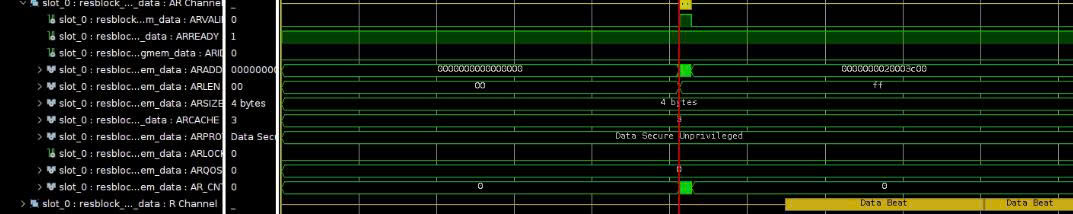
\includegraphics[width=1\linewidth]{Images/waveform.jpg}
%     \caption{Input data waveform of the generator block}
%     \label{fig:gan_waveform}
% \end{figure}
% \begin{figure}[H]
%     \centering
%     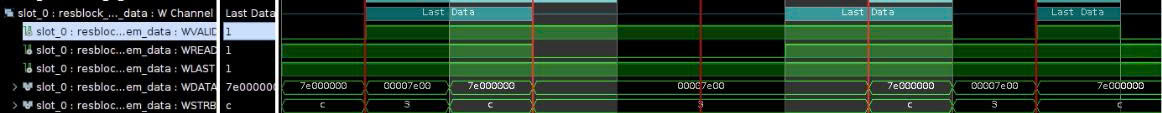
\includegraphics[width=1\linewidth]{Images/wave_w.jpg}
%     \caption{Output data waveform of the generator block}
%     \label{fig:gan_weight_waveform}
% \end{figure}

%%%%%%%%%%%%%%%%%%%%%%%%%%%%%%%%%%%%%%%%%%%%%%%%%%%%%%%%%%%%%%%%%%%%%%%%%%%%%%%%%%%
\subsection{Resource Utilization and Power Considerations}

After functional verification, the complete generator accelerator was synthesized and implemented on the ZCU104 FPGA platform to evaluate resource utilization. The implementation result reflects the cost of mapping all three generator stages (Fusion, UpConv, and Conv77), their local buffering, AXI-based data movement, and control logic into the Programmable Logic (PL). The target clock frequency is 300~MHz, and the implemented design closes timing with a maximum frequency of 308.74~MHz.

The hardware utilization report is summarized in Table~\ref{tab:hific_generator_utilization}. The implemented accelerator uses 205,233 LUTs, corresponding to 89\% of the available LUT resources, and approximately 189,763 FFs, corresponding to 41\% of the available flip-flop resources. For on-chip storage, the design consumes 510 BRAM 18Kb blocks, or 82\% of the available BRAM resources, together with all 96 URAM blocks (100\%). The arithmetic datapath uses 1,550 DSP slices, corresponding to 90\% of the available DSP resources.

\begin{table}[H]
    \centering
    \caption{Hardware resource utilization of the full HiFiC generator accelerator on the ZCU104}
    \label{tab:hific_generator_utilization}
    \begin{tabular}{|l|c|}
        \hline
        \textbf{Resource} & \textbf{Full Generator Accelerator} \\
        \hline
        LUTs & 205,233 (89\%) \\
        \hline
        FFs & 189,763 (41\%) \\
        \hline
        BRAMs (18Kb Block) & 510 (82\%) \\
        \hline
        URAMs & 96 (100\%) \\
        \hline
        DSPs & 1,550 (90\%) \\
        \hline
        Max frequency (MHz) & 308.74 \\
        \hline
    \end{tabular}
\end{table}

The utilization results show that the proposed accelerator is both computation-intensive and memory-intensive. DSP utilization is high because convolution dominates the generator workload and requires a large number of multiply--accumulate operations. BRAM and URAM utilization are also high because intermediate feature maps, line buffers, weights, the up-convolution row accumulator, and the skip-connection buffers must be stored locally to reduce external DDR access and sustain the pipelined datapath; in particular, all available URAM blocks are used.

To show how each core contributes to the overall cost, Table~\ref{tab:resource_breakdown} reports the per-core resource utilization (absolute count and the corresponding share of the device resources). The Fusion and UpConv cores dominate DSP usage because they perform the bulk of the multiply--accumulate work, whereas the Conv77 core is comparatively LUT-heavy due to its final \texttt{Clip}$(0,1)$ stage. The URAM blocks are concentrated in the UpConv core, which stores the row accumulator and the sliding-window buffers required by the transposed convolution.

\begin{table}[H]
    \centering
    \caption{Per-core resource utilization of the generator accelerator}
    \label{tab:resource_breakdown}
    \small
    \setlength{\tabcolsep}{4pt}
    \renewcommand{\arraystretch}{1.2}
    \begin{tabular}{|l|c|c|c|c|c|}
        \hline
        \textbf{Core} & \textbf{BRAM\_18K} & \textbf{DSP} & \textbf{FF} & \textbf{LUT} & \textbf{URAM} \\
        \hline
        Fusion Core & 208 (33\%) & 558 (32\%) & 62,081 (13\%) & 51,574 (22\%) & 16 (17\%) \\
        \hline
        UpConv Core & 144 (23\%) & 576 (33\%) & 56,246 (12\%) & 45,921 (20\%) & 36 (38\%) \\
        \hline
        Conv77 Core & 56 (9\%) & 448 (26\%) & 41,896 (9\%) & 69,081 (30\%) & 0 (0\%) \\
        \hline
        Other / overhead & 193 (31\%) & 32 (2\%) & 15,521 (3\%) & 15,798 (7\%) & 16 (17\%) \\
        \hline
        \textbf{Total} & \textbf{601 (96\%)} & \textbf{1,614 (93\%)} & \textbf{175,744 (38\%)} & \textbf{182,374 (79\%)} & \textbf{68 (71\%)} \\
        \hline
    \end{tabular}
\end{table}

In Table~\ref{tab:resource_breakdown}, the percentage in each cell is taken relative to the resources available on the XCZU7EV device (624 BRAM\_18K, 1{,}728 DSP, 460{,}800 FF, 230{,}400 LUT, and 96 URAM). The figures correspond to the synthesis estimate of each core before the final data-buffer rebalancing step (PIPO double-buffering), which redistributes storage between BRAM and URAM and moves part of the FP16 multipliers from the DSP slices to LUT fabric without changing functionality. The fully implemented design therefore closes at the slightly different resource figures reported in Table~\ref{tab:hific_generator_utilization} (1,550 DSPs, 510 BRAMs, all 96 URAMs, and 205,233 LUTs).

On-board power was not measured in this work; a quantitative power evaluation is left for future board-level deployment. Qualitatively, the main contributors to dynamic power are DSP activity, BRAM/URAM access, AXI memory transfers, and clocked control logic, so reducing unnecessary memory movement and improving data reuse are important not only for performance but also for power efficiency. As an order-of-magnitude reference, the ZCU104 programmable logic typically operates within an envelope of roughly 8--15~W for designs at this utilization, about an order of magnitude below desktop- and laptop-class GPUs ($\sim$60--80~W). This favorable power envelope, rather than raw wall-clock latency, is the basis for the performance-per-watt argument discussed in the comparison below.

%%%%%%%%%%%%%%%%%%%%%%%%%%%%%%%%%%%%%%%%%%%%%%%%%%%%%%%%%%%%%%%%%%%%%%%%%%%%%%%%%%%
\subsection{Performance Evaluation}

In addition to resource utilization, several performance metrics are used to evaluate the effectiveness of the proposed accelerator. These metrics include operating frequency, throughput, accelerated block, numerical precision, and speedup compared with the software-only baseline.

Table~\ref{tab:performance_evaluation} summarizes the main performance results. The accelerator operates at 300~MHz and implements the complete HiFiC generator. The total compute volume of the generator is 90.34~GOP (counting the operations actually executed by the MAC engines), and the design processes one $256\times256$ image in 735.6~ms, giving a sustained throughput of 122.8~GOPS. The latency is dominated by the Fusion Core (568.8~ms), followed by the UpConv Core (149.0~ms) and the Conv77 Core (17.75~ms).

\begin{table}[H]
    \centering
    \caption{Performance evaluation of the proposed accelerator}
    \label{tab:performance_evaluation}
    \begin{tabular}{|l|c|}
        \hline
        \textbf{Metric} & \textbf{Result} \\
        \hline
        FPGA platform & ZCU104 (XCZU7EV) \\
        \hline
        Operating frequency & 300~MHz (Fmax 308.74~MHz) \\
        \hline
        Accelerated network & Full HiFiC generator \\
        \hline
        Precision & Mixed FP16 \\
        \hline
        Compute volume & 90.34~GOP \\
        \hline
        Total latency (per image) & 735.6~ms \\
        \hline
        Throughput & 122.8~GOPS \\
        \hline
    \end{tabular}
\end{table}

The total workload of the generator and its distribution across blocks are summarized in Table~\ref{tab:compute_volume}. The MAC count is derived directly from the tensor dimensions, using
\[
\text{MACs}_{\text{conv}} = H_{out}\,W_{out}\,C_{out}\,C_{in}\,K_H\,K_W,
\qquad
\text{MACs}_{\text{convT}} = H_{in}\,W_{in}\,C_{in}\,C_{out}\,K_H\,K_W,
\]
for standard and transposed convolution, respectively. The nine residual blocks dominate the workload with 38.22~GMAC, whereas the four up-convolution blocks each contribute an identical 1.062~GMAC: although every UCB halves the channel count, it quadruples the spatial resolution, so the transposed-convolution MAC count remains constant across the four stages.

\begin{table}[H]
    \centering
    \caption{Compute volume (MAC operations) of the generator blocks}
    \label{tab:compute_volume}
    \small
    \renewcommand{\arraystretch}{1.2}
    \begin{tabular}{|l|c|c|c|c|}
        \hline
        \textbf{Block} & \textbf{$C_{in}\rightarrow C_{out}$} & \textbf{Spatial out} & \textbf{Kernel} & \textbf{MACs} \\
        \hline
        CBI & $220\rightarrow960$ & $16\times16$ & $3\times3$ & 2.123~G \\
        \hline
        ResBlock $\times 9$ & $960\rightarrow960$ & $16\times16$ & $3\times3$ & 38.220~G \\
        \hline
        GlobalAdd & --- & $16\times16$ & --- & $\sim0$ \\
        \hline
        UCB\_0 & $960\rightarrow480$ & $32\times32$ & $3\times3$ & 1.062~G \\
        \hline
        UCB\_1 & $480\rightarrow240$ & $64\times64$ & $3\times3$ & 1.062~G \\
        \hline
        UCB\_2 & $240\rightarrow120$ & $128\times128$ & $3\times3$ & 1.062~G \\
        \hline
        UCB\_3 & $120\rightarrow60$ & $256\times256$ & $3\times3$ & 1.062~G \\
        \hline
        Conv77 & $60\rightarrow3$ & $256\times256$ & $7\times7$ & 0.578~G \\
        \hline
        \textbf{Total} & & & & \textbf{45.17~GMAC (90.34~GOP)} \\
        \hline
    \end{tabular}
\end{table}

The latency of the design is deterministic and is obtained from the per-loop synthesis report multiplied by the actual trip counts. Table~\ref{tab:latency_breakdown} lists the cycle count and the corresponding latency at 300~MHz for each stage. The Fusion Core accounts for the largest share (568.8~ms), driven by the nine residual blocks; the UpConv Core takes 149.0~ms after the dataflow optimization, and the Conv77 Core completes in about 17.75~ms.

\begin{table}[H]
    \centering
    \caption{Latency breakdown of the generator stages at 300~MHz}
    \label{tab:latency_breakdown}
    \small
    \renewcommand{\arraystretch}{1.2}
    \begin{tabular}{|l|l|c|c|}
        \hline
        \textbf{Stage} & \textbf{Component} & \textbf{Cycles} & \textbf{Latency} \\
        \hline
        \multirow{3}{*}{Fusion} & CBI & 8,980,370 & 29.93~ms \\
        \cline{2-4}
         & ResBlock $\times 9$ & 161,646,705 & 538.82~ms \\
        \cline{2-4}
         & GlobalAdd & 15,507 & 0.05~ms \\
        \hline
        UpConv & $4\times$ UCB (after dataflow opt.) & 44,700,000 & 149.0~ms \\
        \hline
        Conv77 & Conv $7\times7$ + Clip & 5,325,000 & 17.75~ms \\
        \hline
        \multicolumn{2}{|l|}{\textbf{Total (per image)}} & \textbf{220,667,582} & \textbf{735.6~ms} \\
        \hline
    \end{tabular}
\end{table}

Finally, Table~\ref{tab:throughput_breakdown} reports the sustained throughput and the MAC-array efficiency of each core, computed as the ratio between the achieved and the peak MAC rate. The Fusion Core reaches 141.9~GOPS at about 92\% MAC efficiency thanks to the rotating accumulator that sustains an initiation interval of one; the UpConv Core reaches 57.0~GOPS (74\%), and the Conv77 Core 65.1~GOPS. The lower efficiency of the Conv77 Core is expected because it processes a comparatively small workload (0.578~GMAC) whose latency is dominated by pipeline fill/drain and boundary padding rather than by the MAC array. Aggregated over the sequential execution of the three stages, the design sustains 122.8~GOPS.

\begin{table}[H]
    \centering
    \caption{Per-core throughput and MAC-array efficiency at 300~MHz}
    \label{tab:throughput_breakdown}
    \small
    \renewcommand{\arraystretch}{1.2}
    \begin{tabular}{|l|c|c|c|c|c|}
        \hline
        \textbf{Core} & \textbf{Peak MAC/cy} & \textbf{Peak GOPS} & \textbf{Latency} & \textbf{Achieved GOPS} & \textbf{MAC eff.} \\
        \hline
        Fusion & 256 & 153.6 & 568.8~ms & 141.9 & 92\% \\
        \hline
        UpConv & 128 & 76.8 & 149.0~ms & 57.0 & 74\% \\
        \hline
        Conv77 & 448 & 268.8 & 17.75~ms & 65.1 & 24\% \\
        \hline
        \textbf{Full generator} & --- & --- & \textbf{735.6~ms} & \textbf{122.8} & --- \\
        \hline
    \end{tabular}
\end{table}

The performance result shows that the accelerator benefits from parallel DSP computation and local on-chip buffering. The Fusion Core, which executes the convolution-heavy residual blocks, reaches about 92\% of its peak MAC throughput thanks to the rotating accumulator and the overlapped convolution and normalization passes; the UpConv and Conv77 cores are less MAC-bound because their latency also includes pipeline fill/drain and boundary handling. The high BRAM, URAM, and DSP utilization indicates that further performance scaling must be balanced carefully against the remaining device resources.

%%%%%%%%%%%%%%%%%%%%%%%%%%%%%%%%%%%%%%%%%%%%%%%%%%%%%%%%%%%%%%%%%%%%%%%%%%%%%%%%%%%
\subsection{Comparison}

To the best of our knowledge, the HiFiC model has not previously been implemented on an FPGA, so there is no prior hardware accelerator of the same model to compare against directly. Therefore, this section evaluates the proposed accelerator by comparing its performance against the software execution baseline, focusing on the acceleration ratio (speedup) and throughput.

The software baseline corresponds to the full generator inference profiled on an Intel Core i9 CPU operating at 2.2~GHz, which takes 1073.19~s per image, as reported in the runtime breakdown of Table~\ref{tab:runtime_breakdown} in Chapter~3. This baseline is a single-threaded, unoptimized C reference implementation that also serves as the functional golden model; its long runtime is a direct consequence of the very large feature tensors of the generator (for example, $16\times16\times960$ inside each residual block) combined with the absence of multi-threading and vectorization. The proposed accelerator executes the same generator on the ZCU104 platform at 300~MHz in 735.6~ms using mixed FP16 precision. For additional context, the same generator was also profiled on a desktop-class GPU (NVIDIA RTX~3060 Laptop, FP32), which completes one image in 25.1~ms. Table~\ref{tab:performance_comparison} summarizes the comparison.

\begin{table}[H]
    \centering
    \caption{Performance comparison between the software baseline and the proposed FPGA accelerator}
    \label{tab:performance_comparison}
    \begin{tabular}{|>{\raggedright\arraybackslash}p{2.6cm}|>{\raggedright\arraybackslash}p{3.6cm}|c|c|c|}
        \hline
        \textbf{Platform} & \textbf{Device} & \textbf{Precision} & \textbf{Latency} & \textbf{Speedup} \\
        \hline
        Software (CPU, single-thread ref.) & Intel Core i9 @ 2.2~GHz & FP32 & 1073.19~s & $1\times$ \\
        \hline
        GPU (desktop-class) & NVIDIA RTX 3060 Laptop & FP32 (cuDNN) & 25.1~ms & $\approx 42{,}700\times$ \\
        \hline
        Proposed FPGA & ZCU104 (XCZU7EV) @ 300~MHz & Mixed FP16 & 735.6~ms & $\approx 1459\times$ \\
        \hline
    \end{tabular}
\end{table}

The comparison shows that running the full generator on the FPGA reduces the per-image processing time from 1073.19~s on the CPU to 735.6~ms, an acceleration of approximately $1459\times$, while sustaining a throughput of 122.8~GOPS. This large speedup is obtained even though the FPGA operates at a much lower clock frequency than the CPU, because the accelerator exploits spatial parallelism through many processing elements, local on-chip buffering, and overlapped convolution and normalization passes that keep the MAC datapath busy. The result confirms that dedicated hardware is essential for the compute-bound HiFiC generator, whose very large feature tensors make plain CPU execution impractical.

It should be emphasized that these speedup ratios are measured against the single-threaded, unoptimized reference C implementation and therefore quantify acceleration over that specific software reference rather than over peak-optimized software. An optimized, multi-threaded CPU library (for example, oneDNN) executes the same generator in a few hundred milliseconds, comparable to the FPGA, and a desktop-class GPU is faster still in raw wall-clock time (25.1~ms). The proposed accelerator is therefore not positioned as the fastest wall-clock platform; its advantage lies in deterministic, low-latency inference within an embedded power envelope (programmable-logic power on the order of 8--15~W, against roughly 60--80~W for the GPU), that is, a favorable performance-per-watt for resource-constrained deployment. A full performance-per-watt comparison based on on-board power measurement is left for future work.

%%%%%%%%%%%%%%%%%%%%%%%%%%%%%%%%%%%%%%%%%%%%%%%%%%%%%%%%%%%%%%%%%%%%%%%%%%%%%%%%%%%
\subsection{Chapter Conclusion}

Chapter 4 presented the experimental results of the proposed quantized HiFiC GAN accelerator. Block-level C-simulation against the FP32 golden reference passed with zero element mismatches across all generator stages, and the accuracy evaluation further compared the HLS simulation output with the Python reference model using PSNR over 100 test images; the mixed-precision quantization results showed that compression ratio, PSNR, and SSIM are preserved when moving from FP32 to FP16. The resource utilization report showed that the design uses a large portion of the available DSP, BRAM, and URAM resources (all URAM blocks are used), which is expected for a highly parallel full-generator accelerator. The performance evaluation demonstrated an operating frequency of 300~MHz (timing closed at 308.74~MHz), a total compute volume of 90.34~GOP, a total latency of 735.6~ms per image (568.8~ms Fusion, 149.0~ms UpConv, 17.75~ms Conv77), a throughput of 122.8~GOPS, and an acceleration of approximately $1459\times$ over the CPU software baseline.

Overall, the results confirm that the proposed hardware--software co-design is suitable for accelerating the complete HiFiC generator while preserving reconstruction quality.
